
\section{Optimisation}

\begin{frame}
	\frametitle{Key components for image classification}

	\begin{enumerate}
		\item score function
		\item loss function
		\item optimisation
	\end{enumerate}

	Optimisation is the process of finding the set of parameters $W$ that 
	minimise the loss function $L$.

\end{frame}

\begin{frame}
	\frametitle{Visualising the loss function}

	If $W_0$ random starting point, $W_1$ random direction, then compute 
	$L(W_0 + a W_1)$ for different values of $a$.

	\centering
        \begin{figure}
                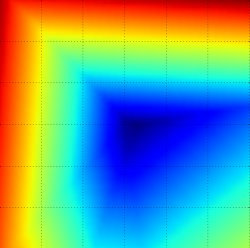
\includegraphics[width=0.4\textwidth]{Pics/svm_one.jpg}
        \end{figure}
	
	\small{(averaged across all images, $x_i$)}

\end{frame}

\begin{frame}
	\frametitle{Optimisation}

	\begin{columns}
		
		\column{0.3\textwidth}
		\begin{figure}
	                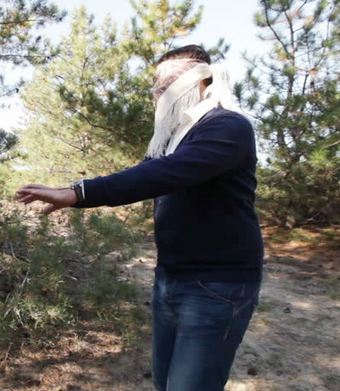
\includegraphics[width=0.8\textwidth]{Pics/hiker.png}
        	\end{figure}
		\column{0.7\textwidth}
		\begin{itemize}
			\item Random search
			\item Random local search
			\item Gradient descent (numerical or analytical)
		\end{itemize}

	\end{columns}

	\vskip 1cm
	\begin{equation*}
		\frac{df(x)}{dx} = \lim_{h \rightarrow 0} \frac{f(x+h)-f(x)}{h}
	\end{equation*}

\end{frame}

\begin{frame}
	\frametitle{Hyperparameters}

	\begin{columns}
		\column{0.5\textwidth}
		\textbf{Step size} or learning rate
		\centering
		\begin{figure}
                	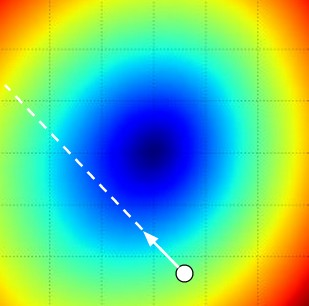
\includegraphics[width=0.8\textwidth]{Pics/stepsize.jpg}
        	\end{figure}
		\column{0.5\textwidth}
		\textbf{Batch size}:\\
		Compute the gradient over batches (e.g. 32, 64, 128...) of the 
		training data.
	\end{columns}

\end{frame}

\begin{frame}
	\frametitle{Backpropagation}

	We can compute the gradient analytically using the chain rule.

	\vskip 0.5cm

	\centering
	$f(x,y,z)=(x+y)z$\\
	$q=x+y$ and $f=qz$\\
	$\frac{df}{dx}=\frac{df}{dq}\frac{dq}{dx}$

        \begin{figure}
                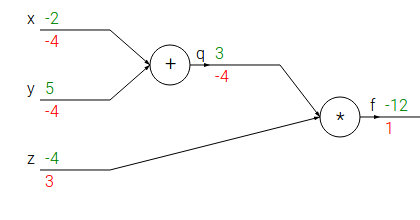
\includegraphics[width=0.6\textwidth]{Pics/backpropagation}
        \end{figure}

\end{frame}


\begin{frame}
	\frametitle{Wrap up}

	\centering
	\begin{figure}
        	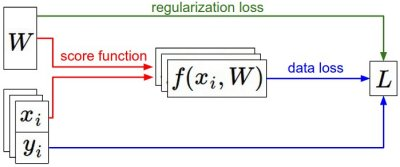
\includegraphics[width=0.6\textwidth]{Pics/dataflow.jpeg}
      	\end{figure}

	The 3 elements: score function, loss function, optimisation.

	Next: let's put them all together in a neural network.

\end{frame}















